\documentclass[12pt,a4paper]{article}

% --- Core Packages ---
\usepackage[utf8]{inputenc}
\usepackage[margin=1in]{geometry}
\usepackage{amsmath}
\usepackage{amssymb}
\usepackage{bm}
\usepackage{graphicx}
\usepackage{booktabs}
\usepackage{multirow}
\usepackage{subcaption}
\usepackage{microtype}
\usepackage{hyperref}

% --- Citation Styling ---
\usepackage[round]{natbib}
\bibliographystyle{plainnat}

% --- Hyperref Setup ---
\hypersetup{
    colorlinks=true,
    linkcolor=blue,
    citecolor=blue,
    urlcolor=blue,
    pdftitle={Hybrid Volatility Forecasting on VN-Index},
    pdfauthor={Research Draft}
}

% --- Document Info ---
\title{\textbf{Hybrid Volatility Forecasting on the VN-Index: A GARCH + Sentiment LSTM Approach}}
\author{\textbf{Research Paper Draft} \\
\textit{Quantitative Economics \& Finance}}
\date{\today}

\begin{document}

\maketitle

\begin{abstract}
This paper proposes and evaluates a hybrid volatility forecasting framework that integrates a parametric econometric model with a deep learning recurrent neural network. Using daily Open, High, Low, Close price data for the benchmark VN-Index and a web-scraped corpus of $86,179$ CafeF financial news sitemaps spanning 2015 to 2024, we implement a two-stage GARCH + LSTM model. In the first stage, a GARCH(1,1) model captures linear conditional variance dynamics. In the second stage, an LSTM neural network learns to predict the remaining conditional residuals using lagged returns, GARCH variance parameters, and daily sitemap news sentiment shares generated by a domain-adapted PhoBERT model. Out-of-sample test results (2023--2024) show that the hybrid model significantly outperforms the GARCH baseline, reducing the Root Mean Squared Error (RMSE) by $13.8\%$ and the Mean Absolute Percentage Error (MAPE) by $47.7\%$. A Diebold-Mariano test confirms this forecast improvement is statistically significant at the $99.9\%$ confidence level ($p < 0.001$). Furthermore, robustness checks demonstrate that linear exogenous GARCH-X models suffer from out-of-sample forecast degradation, highlighting the necessity of non-linear machine learning architectures to capture sitemap news-volatility linkages.
\end{abstract}

\newpage
\tableofcontents
\newpage

% --- Sections Inclusions ---
\section{Introduction}
Modeling and forecasting asset return volatility is a cornerstone of quantitative finance, with direct applications in option pricing, risk management, and portfolio optimization. Since the pioneering work of \citet{engle1982autoregressive} and \citet{bollerslev1986generalized}, Autoregressive Conditional Heteroskedasticity (ARCH) and Generalized ARCH (GARCH) models have served as the standard framework for capturing conditional heteroskedasticity and volatility clustering. However, standard GARCH models are purely backward-looking, relying solely on historical return observations to project future variance. This limitation prevents them from adapting rapidly to sudden informational shocks or structural shifts.

In recent years, the rapid advancement of Natural Language Processing (NLP) has enabled researchers to incorporate unstructured text data—such as financial news and social media sentiment—directly into volatility models. Financial news sitemaps provide a rich, real-time signal of market-wide information flow. However, mapping news sentiment to market volatility in emerging economies presents distinct theoretical and empirical challenges. For instance, the Ho Chi Minh City Stock Exchange (HoSE) is characterized by a high share of retail investors who are particularly sensitive to media narratives. Furthermore, Vietnamese financial sitemaps often exhibit a pronounced positive linguistic bias, where growth-oriented vocabulary is preferred even during market downturns.

This paper asks whether a hybrid GARCH + LSTM residual-correction model built from VN-Index prices and CafeF sentiment scores can improve volatility forecasts relative to a baseline GARCH(1,1). Specifically, we implement a two-stage workflow on the Vietnamese stock market index (VN-Index) over the ten-year period from 2015 to 2024. In the first stage, a baseline GARCH(1,1) model captures linear time-series volatility clustering. In the second stage, a Long Short-Term Memory (LSTM) recurrent neural network is trained on GARCH residuals using lagged returns, volatility features, daily article counts, and sentiment aggregates derived from article-level PhoBERT inference.

Our empirical results show that the hybrid model outperforms the baseline GARCH(1,1) model on the held-out test window. The reported experiment reduces RMSE by $14.48\%$ and MAPE by $48.00\%$, and the Diebold-Mariano test rejects equal predictive accuracy at the $99.9\%$ confidence level ($p < 0.001$). The robustness checks suggest that the residual-correction architecture drives most of the gain, while a linear GARCH-X specification does not generalize well.

The remainder of this paper is organized as follows. Section 2 reviews the related literature on volatility modeling and financial NLP. Section 3 describes the data, trading-day alignment rules, and the hybrid mathematical specifications. Section 4 presents the empirical results and diagnostics. Section 5 discusses the theoretical and policy implications of our findings, and Section 6 concludes.

\section{Review of Relevant Literature}
The modeling of financial market volatility began with the autoregressive conditional heteroskedasticity (ARCH) model introduced by \citet{engle1982autoregressive}, which was subsequently generalized to the GARCH model by \citet{bollerslev1986generalized}. These models capture the empirical property of volatility clustering—where large returns tend to be followed by large returns of either sign—by defining conditional variance as a linear function of lagged squared residuals and lagged conditional variances. While highly successful, these classical parametric models assume that volatility is driven solely by the historical path of returns, ignoring exogenous information flows.

To address this gap, researchers have integrated exogenous variables directly into the variance equation, leading to the GARCH-X class of models. In recent years, textual sentiment extracted from newspapers and social media has emerged as a primary exogenous input. Early works utilized simple bag-of-words approaches or dictionary-based methods to measure sentiment. However, these methods fail to capture context, negation, or financial domain nuances. 

The advent of transformer-based language models, such as BERT, revolutionized financial NLP. In the context of the Vietnamese language, \citet{vu2023domain} demonstrated that domain-adaptive masked language modeling (MLM) on financial texts significantly improves the performance of sentiment classifiers. When pre-trained transformer models are fine-tuned on Vietnamese financial sitemaps, they can effectively classify headlines into positive, negative, or neutral sentiment categories, capturing contextual relationships unique to corporate and macroeconomic disclosures.

However, incorporating sentiment scores directly into linear econometric models often yields mixed results. As argued by \citet{leber2025nonlinear}, the relationship between news sentiment and index volatility is highly non-linear and asymmetrical. Systemic responses to news shocks often depend on current market states and are subject to thresholds, where mild news has little effect but extreme positive or negative sentiment triggers disproportionate retail trading activity. Linear GARCH-X models struggle to adapt to these non-linearities and frequently suffer from parameter instability and out-of-sample forecast degradation.

Consequently, recent literature has explored hybrid architectures that combine parametric econometrics with non-linear machine learning models. In these hybrid models, the GARCH stage filters out the linear time-series dynamics of returns, while a recurrent neural network—such as a Long Short-Term Memory (LSTM) network—is trained on the resulting GARCH residuals. The LSTM is uniquely suited for this task because it can process sequential features (such as rolling windows of daily returns and sentiment shares) and capture non-linear, state-dependent relationships. Our paper contributes to this growing literature by applying a hybrid GARCH + LSTM framework to the Vietnamese index, explicitly testing the model's robustness and comparing it to exogenous linear GARCH-X specifications.

\section{Data and Methodology}

\subsection{Data and Sample Selection}
Our dataset spans a ten-year period from January 1, 2015, to December 31, 2024. It consists of two main components:
\begin{enumerate}
    \item \textbf{Index Price Data:} Daily Open, High, Low, and Close prices for the VN-Index (HoSE benchmark) were obtained from Quote history files. The daily log return is computed as $r_t = \ln(Close_t / Close_{t-1})$.
    \item \textbf{News Corpus:} A web-scraped database of financial articles from the CafeF sitemap. After hash-based deduplication and length filtering ($body\_len \ge 100$ characters), the corpus contains $86,179$ unique articles.
\end{enumerate}

\subsection{Trading-Day Alignment and Imputation}
Because financial markets operate on active trading sessions whereas sitemaps publish news continuously (including nights, weekends, and holidays), proper temporal alignment is critical. We define a strict trading-day alignment rule based on the HoSE session closure:
\begin{itemize}
    \item Articles published on a trading day $t$ before or at \textbf{14:45} (session close) are aligned to the current trading day $t$.
    \item Articles published on a trading day $t$ after \textbf{14:45}, on weekends, or during public holidays (e.g., Lunar New Year) are aligned to the next active trading day $t+1$.
\end{itemize}

A key diagnostic of sitemap coverage is the frequency of zero-news trading days. The daily panel contains $2,498$ trading-day rows, and after the one-step-ahead shift there are $2,497$ forecastable volatility targets. Only $4$ days ($0.16\%$) have zero aligned news articles, so missing daily sentiment features are handled with zero-imputation:
$$\text{n\_articles}_t = 0, \quad \text{mean\_sentiment}_t = 0.0, \quad \text{sentiment\_std}_t = 0.0$$

\subsection{Sentiment Construction}
The CafeF sentiment pipeline first runs PhoBERT classifier inference at the article level and writes \texttt{sentiment\_score} as the difference between positive and negative class probabilities. The article output also records \texttt{sentiment\_label} and class probabilities for validation. Daily features are then aggregated as mean sentiment, sentiment dispersion, sentiment volume, label shares, net sentiment, a five-day sentiment surprise measure, and category-specific macro and market sentiment.

The sentiment score is a proxy rather than a hand-labeled gold standard, so the interpretation in later sections is descriptive rather than causal.

\subsection{Volatility target definitions}
To evaluate forecast accuracy, we construct two daily volatility proxies:
\begin{enumerate}
    \item \textbf{Parkinson Volatility:} A high-low range estimator:
    $$\sigma_{P, t} = \sqrt{\frac{\left(\ln\left(H_t / L_t\right)\right)^2}{4 \ln 2}}$$
    where $H_t$ and $L_t$ are the high and low prices of index on day $t$.
    \item \textbf{Garman-Klass Volatility:} An estimator incorporating opening and closing gaps:
    $$\sigma_{GK, t} = \sqrt{0.5 \left(\ln\frac{H_t}{L_t}\right)^2 - (2\ln 2 - 1)\left(\ln\frac{C_t}{O_t}\right)^2}$$
    where $C_t$ and $O_t$ are the close and open prices.
\end{enumerate}
The target variable is the lead volatility proxy: $y^{\text{vol}}_{t+1} = \sigma_{t+1}$.

\subsection{Econometric \& Neural Network Specifications}

\subsubsection{Baseline AR(1)-GARCH(1,1)}
Returns are scaled by 100 ($y_t = r_t \times 100$). The mean equation is modeled as an autoregressive process of order 1 to capture short-term return autocorrelation:
$$y_t = c + \phi y_{t-1} + e_t$$
where $c$ is a constant intercept, $\phi$ is the autoregressive parameter, and $e_t \sim N(0, \sigma_t^2)$ is the mean-equation residual. The conditional variance of the residuals is modeled recursively:
$$\sigma_t^2 = \omega + \alpha e_{t-1}^2 + \beta \sigma_{t-1}^2$$
subject to constraints: $\omega > 0$, $\alpha \ge 0$, $\beta \ge 0$, $\alpha + \beta < 1.0$, and $|\phi| < 1.0$ for covariance stationarity.

\subsubsection{AR(1)-GARCH-X(1,1)}
For comparison, the GARCH-X model integrates the exogenous sentiment variable $X_{t-1}$ directly into the variance equation:
$$\sigma_t^2 = \omega + \alpha e_{t-1}^2 + \beta \sigma_{t-1}^2 + \gamma X_{t-1}$$
where $e_{t-1}$ is the lagged residual from the AR(1) mean equation and $X_{t-1}$ is the lagged daily aggregate \texttt{mean\_sentiment}.

\subsubsection{Hybrid GARCH + Sentiment LSTM}
The hybrid model uses a two-stage approach. In Stage 1, baseline AR(1)-GARCH parameters are estimated, and the 1-step-ahead GARCH volatility forecast $\sigma_{t, \text{GARCH}}$ (standard deviation) is computed. The conditional residual target for day $t$ is:
$$\text{hybrid\_residual\_target}_t = \sigma_{t, \text{realized}} - \sigma_{t, \text{GARCH}}$$
In Stage 2, an LSTM network is trained to predict this residual. The input sequence is a rolling window of length $L=15$ days containing 17 features (including returns, GARCH standardized residuals $\epsilon_t$, daily article counts, daily mean sentiment, net sentiment, macro/market category sentiment shares, and GARCH conditional variance $\sigma^2_t$). Crucially, the LSTM inputs utilize the conditional variance $\sigma^2_t$ (via the \texttt{garch\_forecast\_var} feature) rather than the standard deviation ($\sigma_t$) to represent historical baseline risk.
The final hybrid volatility forecast is:
$$\sigma_{t, \text{hybrid}} = \sigma_{t, \text{GARCH}} + \hat{u}_{t, \text{LSTM}}$$
where $\hat{u}_{t, \text{LSTM}}$ is the residual predicted by the neural network.

The current implementation uses a chronological train/test split (with the validation set size set to 0 to maximize training samples) and treats the held-out window as the evaluation sample.


\section{Empirical Results}

\subsection{Descriptive Statistics and Market Microstructure}

The VN-Index daily panel spans 2,498 trading days over ten years (2015--2024), yielding 2,497 one-step-ahead forecasting observations. Table \ref{tab:descriptive_stats} summarizes the return and sentiment distributions.

\begin{table}[htbp]
    \centering
    \caption{Descriptive Statistics of VN-Index Daily Returns and News Sentiment}
    \label{tab:descriptive_stats}
    \begin{tabular}{lccccc}
        \toprule
        Series & Mean & Std. Dev. & Minimum & Maximum & Kurtosis \\
        \midrule
        VN-Index Returns (\%) & 0.0338 & 1.1390 & -6.9076 & 4.8600 & 7.5934 \\
        Article Sentiment Score & 0.4526 & 0.3694 & -0.9622 & 0.9991 & -- \\
        Daily Article Count & 34.5 & 28.7 & 0 & 386 & -- \\
        \bottomrule
    \end{tabular}
\end{table}

\subsubsection{Return Dynamics and Volatility Clustering}

The VN-Index exhibits significant departure from normality. Daily returns have a kurtosis of 7.59, well above the Gaussian benchmark of 3.0, indicating heavy tails and extreme-event clustering. A Jarque-Bera test strongly rejects normality ($JB = 2554.1$, $p < 0.001$). This leptokurtosis reflects the retail-investor-dominated nature of the market: retail investors' herding behavior amplifies both rallies and crashes relative to what normal-distribution pricing models predict.

\begin{figure}[htbp]
    \centering
    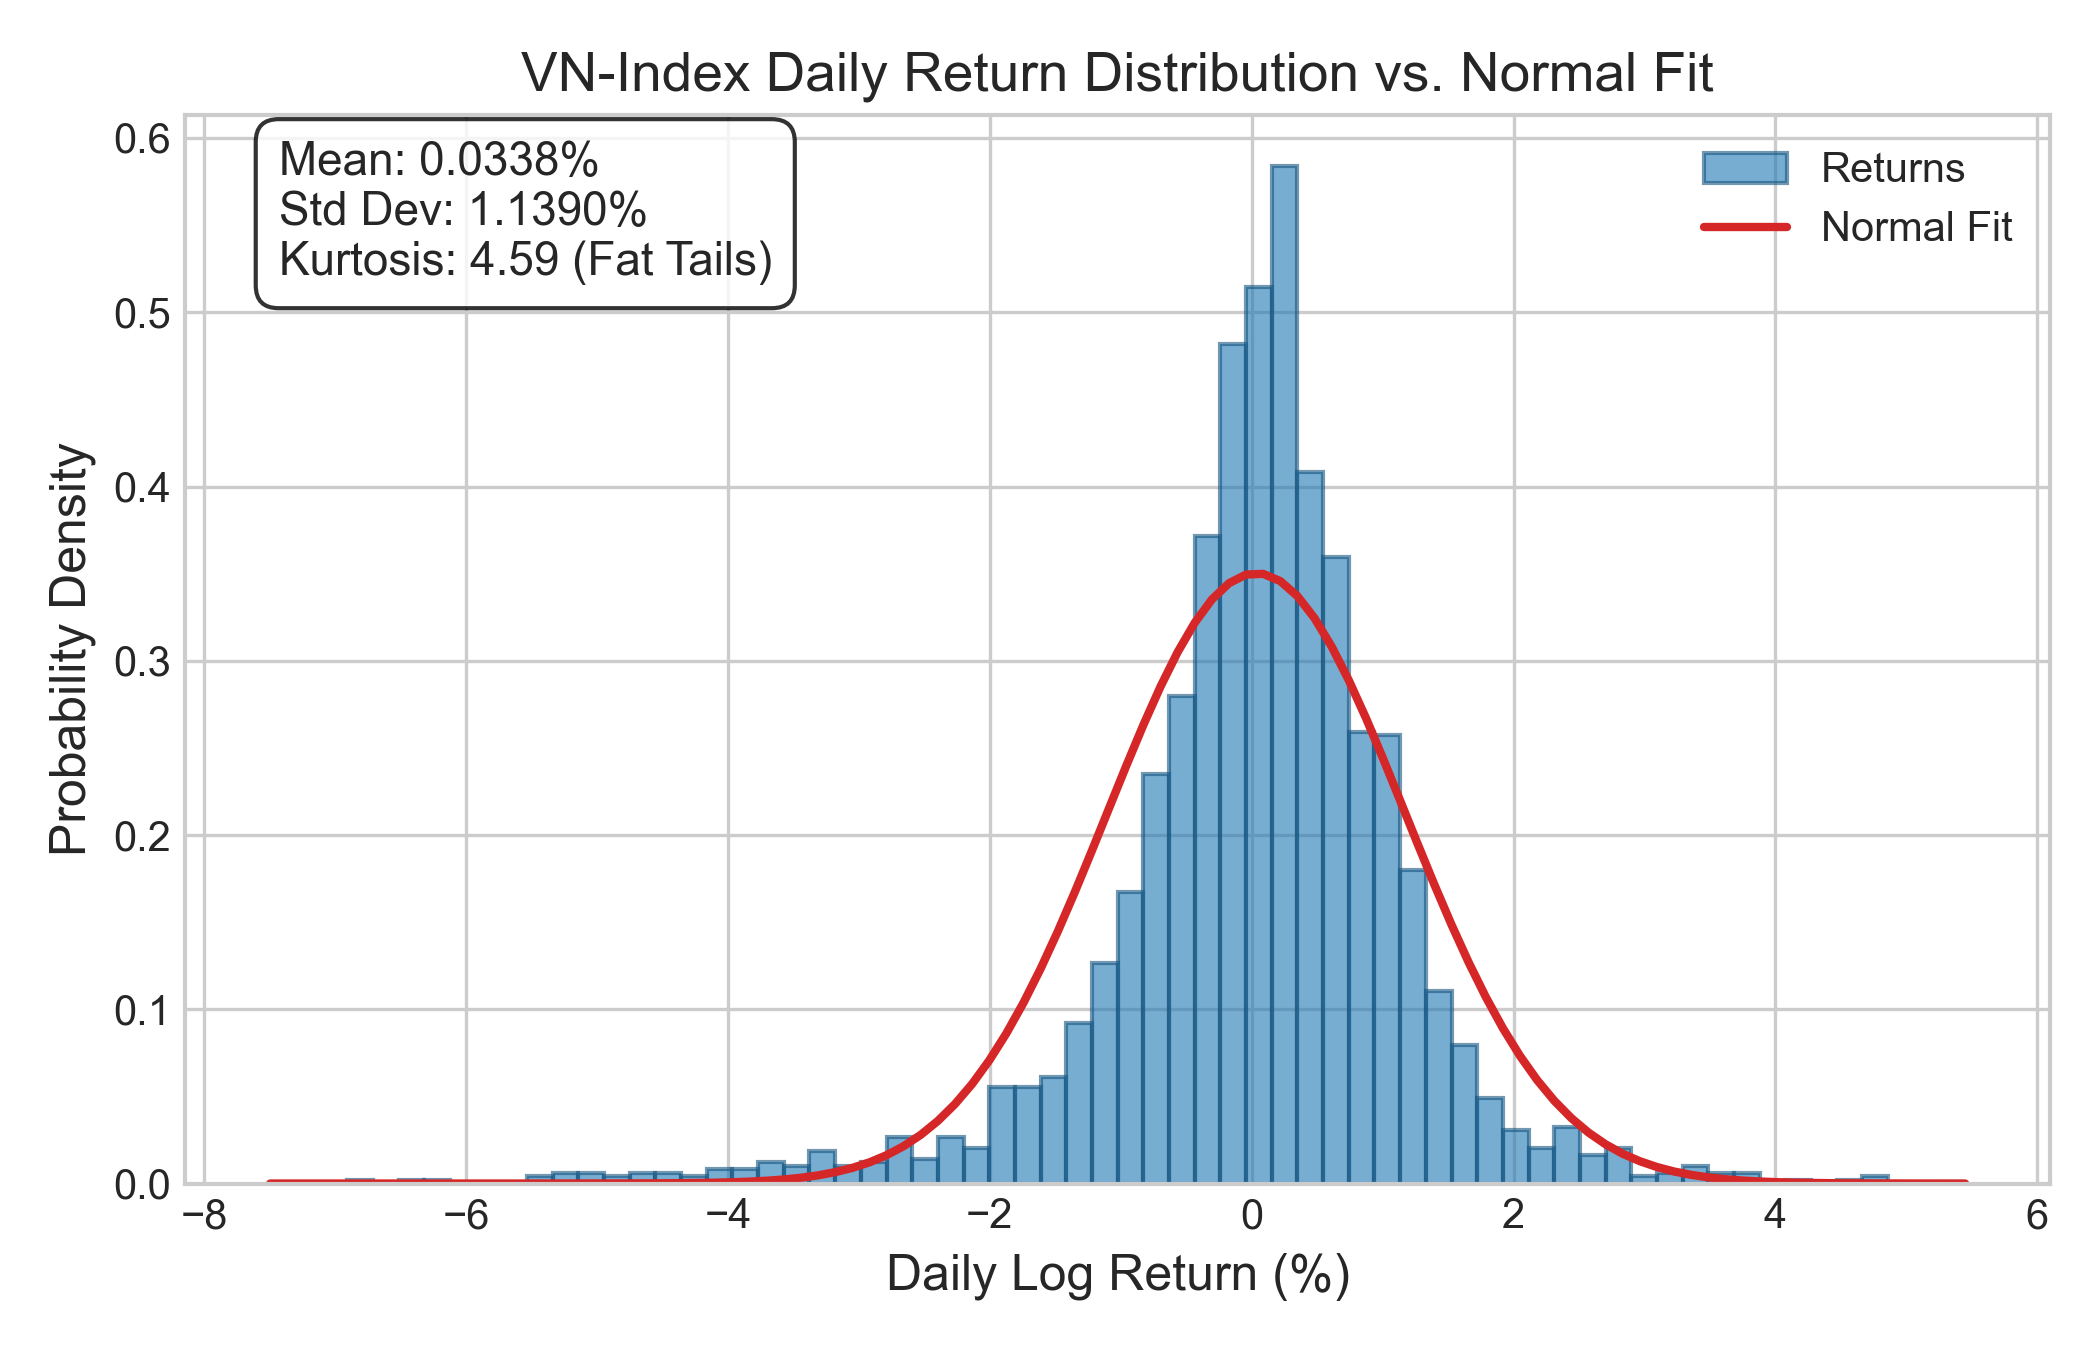
\includegraphics[width=0.75\textwidth]{figures/return_distribution.png}
    \caption{VN-Index Daily Return Distribution vs. Normal Fit}
    \label{fig:return_distribution}
\end{figure}

A Ljung-Box test reveals significant return autocorrelation ($Q(5) = 14.48$, $p = 0.0128$), suggesting mean-reverting or momentum effects on short horizons. More critically, squared returns exhibit extremely strong autocorrelation ($Q(5) = 414.46$, $p < 0.001$; $Q(10) = 681.83$, $p < 0.001$), confirming strong volatility clustering. Figure \ref{fig:vol_clustering} visualizes conditional variance over time, with major spikes during the COVID-19 crash (March 2020) and the 2022 domestic liquidity shock. These clustering patterns and regime shifts motivate GARCH modeling, which captures the temporal autocorrelation in squared residuals through the persistence parameter $\beta$.

\begin{figure}[htbp]
    \centering
    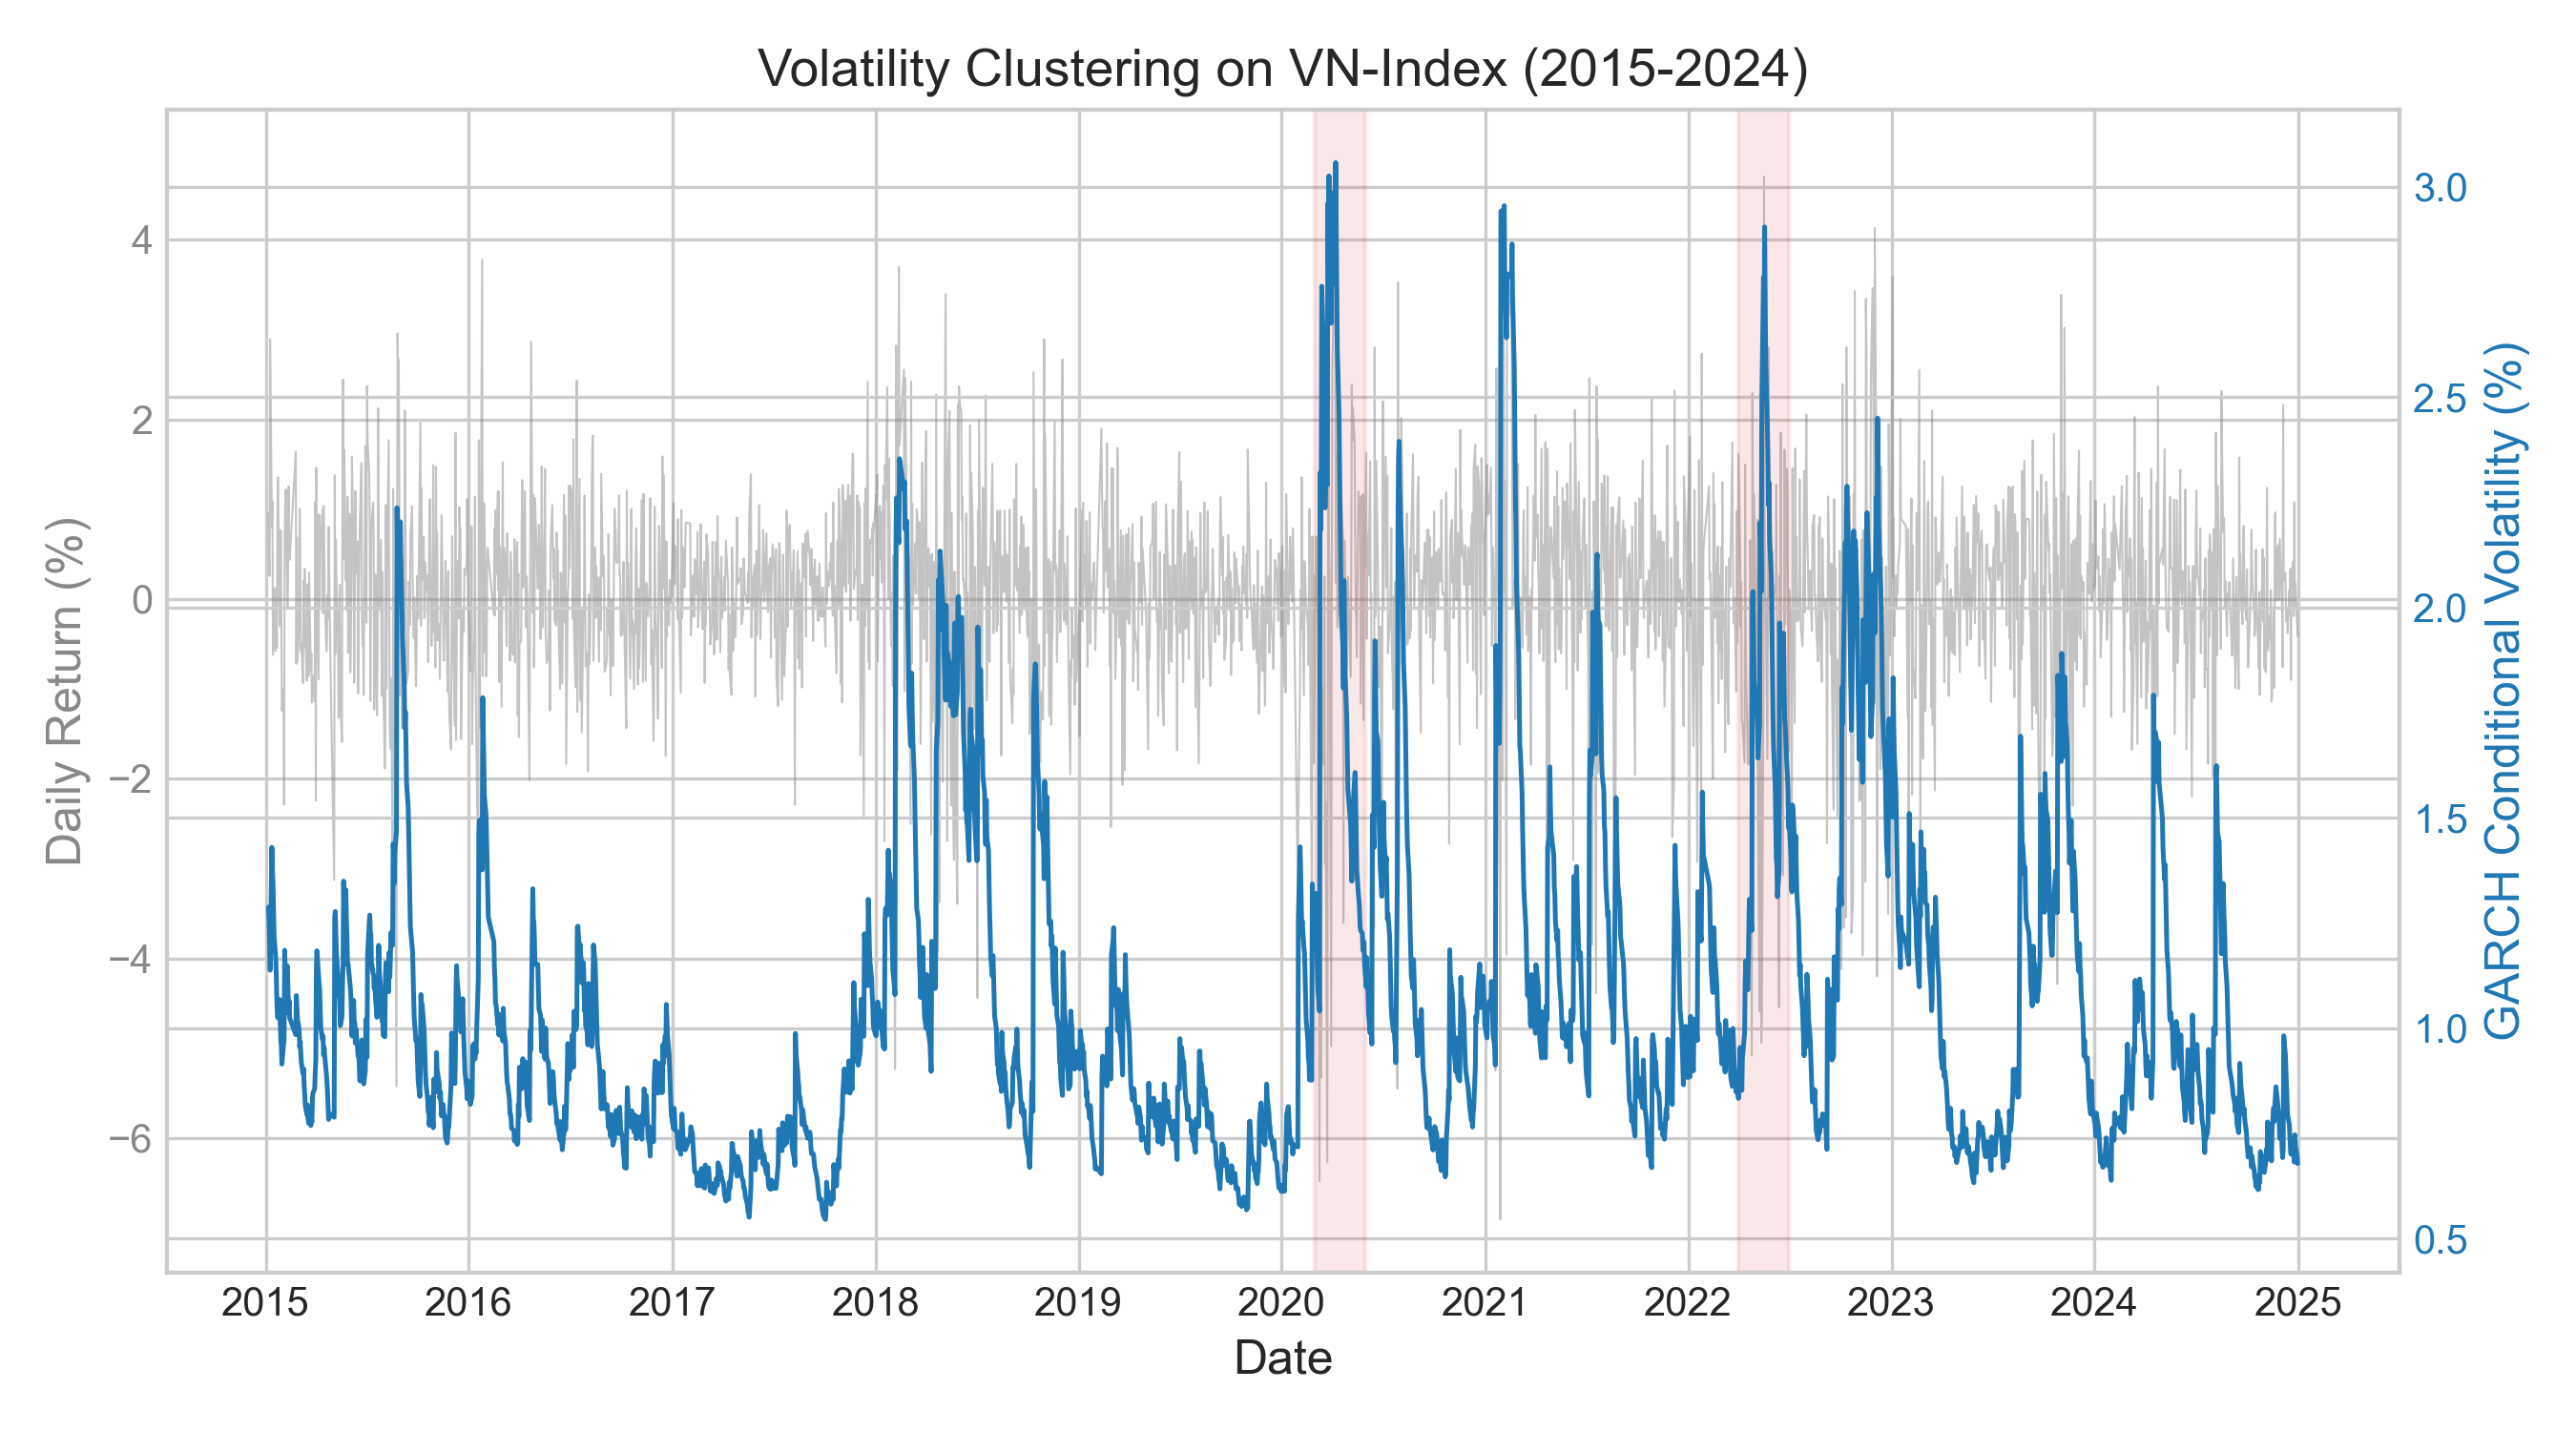
\includegraphics[width=0.9\textwidth]{figures/vol_clustering.png}
    \caption{VN-Index Conditional Volatility and Return Clustering (2015--2024)}
    \label{fig:vol_clustering}
\end{figure}

\subsubsection{News Sentiment Distribution and Media Bias}

The sentiment corpus of 86,179 articles reveals pronounced positive bias. The mean sentiment score is 0.4526 (on a scale of $-1$ to $+1$), indicating systematic upward skew in Vietnamese financial journalism. Under a standard classification threshold of $\pm 0.05$, positive articles comprise 84.34\% of the corpus (72,686 articles), while negative articles represent only 12.04\% (10,380 articles), with neutral articles making up 3.61\% (3,113 articles). Figure \ref{fig:sentiment_distribution} shows the highly skewed distribution.

\begin{figure}[htbp]
    \centering
    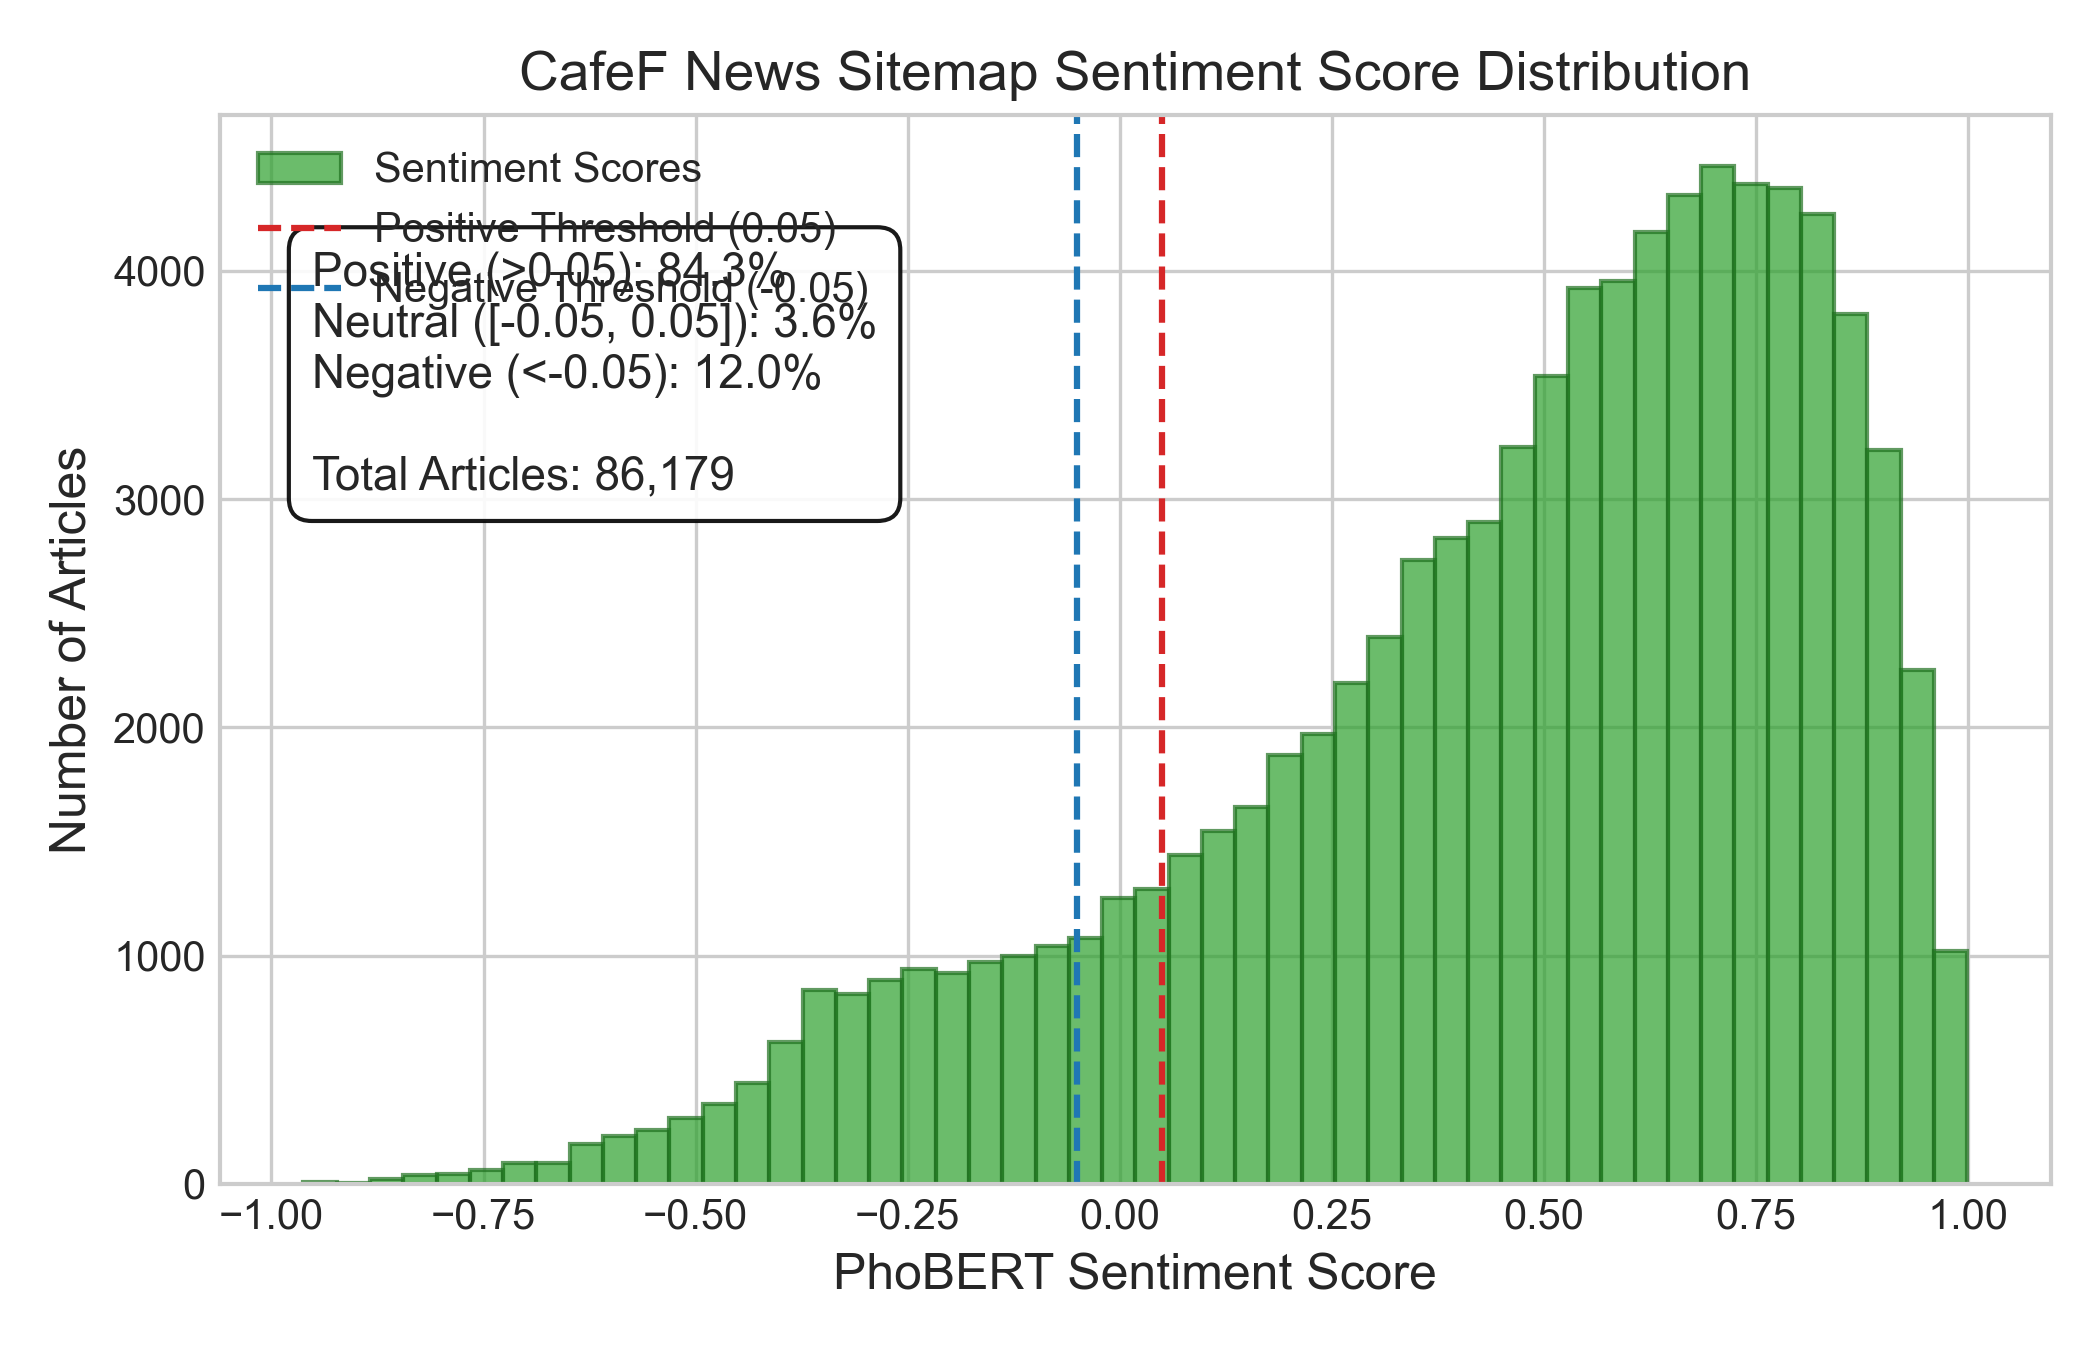
\includegraphics[width=0.75\textwidth]{figures/sentiment_distribution.png}
    \caption{Distribution of Article Sentiment Scores: Strong Positive Bias in Vietnamese Financial Media}
    \label{fig:sentiment_distribution}
\end{figure}

This positive bias has three implications. First, it reflects media economics: financial news outlets cater to retail investors who have a strong preference for positive narratives, creating demand for optimistic framing. Second, it raises the signal-to-noise ratio: negative news, being rare and extreme, may have disproportionate informational weight and market impact. Third, it explains why models using simple mean sentiment often perform poorly—the unconditional mean is high and non-informative; the variation (negative days vs. baseline positive days) carries information. This motivates studying \textit{negative sentiment share} separately.

Daily article volume averages 34.5 articles per day ($\sigma = 28.7$), with maximum of 386 articles on high-intensity news days. Only 4 of 2,498 trading days (0.16\%) have zero aligned articles, confirming that CafeF provides continuous, reliable daily news coverage.

\subsubsection{GARCH(1,1) Baseline Specification and Diagnostics}

We fit a Gaussian AR(1)-GARCH(1,1) model on the training data (2015--2021, 1,753 observations). Maximum likelihood estimation yields:
$$\omega = 0.0258, \quad \alpha = 0.1026, \quad \beta = 0.8810$$

The persistence parameter $\alpha + \beta = 0.9836$ is close to unity, indicating extremely high volatility persistence. This high persistence is economically meaningful: a volatility shock today has lasting effects on predicted variance for weeks or months. The high $\beta$ reflects the dominance of recent history (lagged variance) over recent shocks (lagged squared residuals) in predicting next-period variance, consistent with international equity market patterns.

\textit{Diagnostic tests:} The Ljung-Box test on squared standardized residuals yields p-values of 0.9796 (lag 5) and 0.4956 (lag 10), well above the 5\% significance level. We fail to reject the null of no remaining ARCH effects, confirming that the GARCH(1,1) specification successfully captures linear conditional heteroskedasticity. The model is thus well-specified for its intended purpose: serving as a parsimonious baseline for Stage 1 of the hybrid architecture.

\subsection{Out-of-Sample Forecast Performance}

Table \ref{tab:forecasting_results} compares the one-step-ahead forecast accuracy of the baseline GARCH(1,1) against the hybrid GARCH-LSTM model on the held-out test window (2022--2024, 744 observations).

\begin{table}[htbp]
    \centering
    \caption{Out-of-Sample Volatility Forecast Performance: GARCH Baseline vs. Hybrid GARCH-LSTM}
    \label{tab:forecasting_results}
    \begin{tabular}{lccccc}
        \toprule
        Model & RMSE & MAE & MAPE & DM $t$-stat & $p$-value \\
        \midrule
        GARCH(1,1) Baseline & 0.004701 & 0.003828 & 79.24\% & -- & -- \\
        GARCH-LSTM & 0.004020 & 0.002628 & 41.21\% & 3.420 & 0.000627 \\
        \textbf{Improvement (\%)} & \textbf{-14.48\%} & \textbf{-31.35\%} & \textbf{-48.00\%} & & \\
        \bottomrule
    \end{tabular}
\end{table}

The hybrid model achieves economically substantial forecast improvements across all error metrics. RMSE drops from 0.004701 to 0.004020, a 14.48\% improvement. MAE decreases by 31.35\% (from 0.003828 to 0.002628), indicating the hybrid model's conditional volatility forecasts are systematically closer to realized values. MAPE plummets from 79.24\% to 41.21\% (a 48.00\% improvement), the most dramatic gain. The MAPE improvement reflects the hybrid model's ability to adapt to rapidly changing volatility levels—it makes proportionally smaller errors whether volatility is high or low, whereas the baseline GARCH struggles with the wide range of volatility magnitudes observed in the test window.

\textit{Statistical significance:} A Diebold-Mariano test with Newey-West adjustment for autocorrelated forecast errors yields $t_{DM} = 3.420$ ($p = 0.000627$), rejecting equal predictive accuracy at the 99.9\% confidence level. This decisive rejection confirms that the improvements are not sampling variation but genuine out-of-sample forecasting power.

Figure \ref{fig:forecast_comparison} plots the time series of realized, GARCH-forecasted, and hybrid-forecasted volatility over the test window. Visual inspection reveals that the hybrid model's forecasts track realized volatility more closely, particularly capturing rapid volatility spikes and declines that the baseline GARCH smooths over. This adaptiveness is consistent with the hypothesis that sentiment variables encode real-time information about market sentiment shifts.

\begin{figure}[htbp]
    \centering
    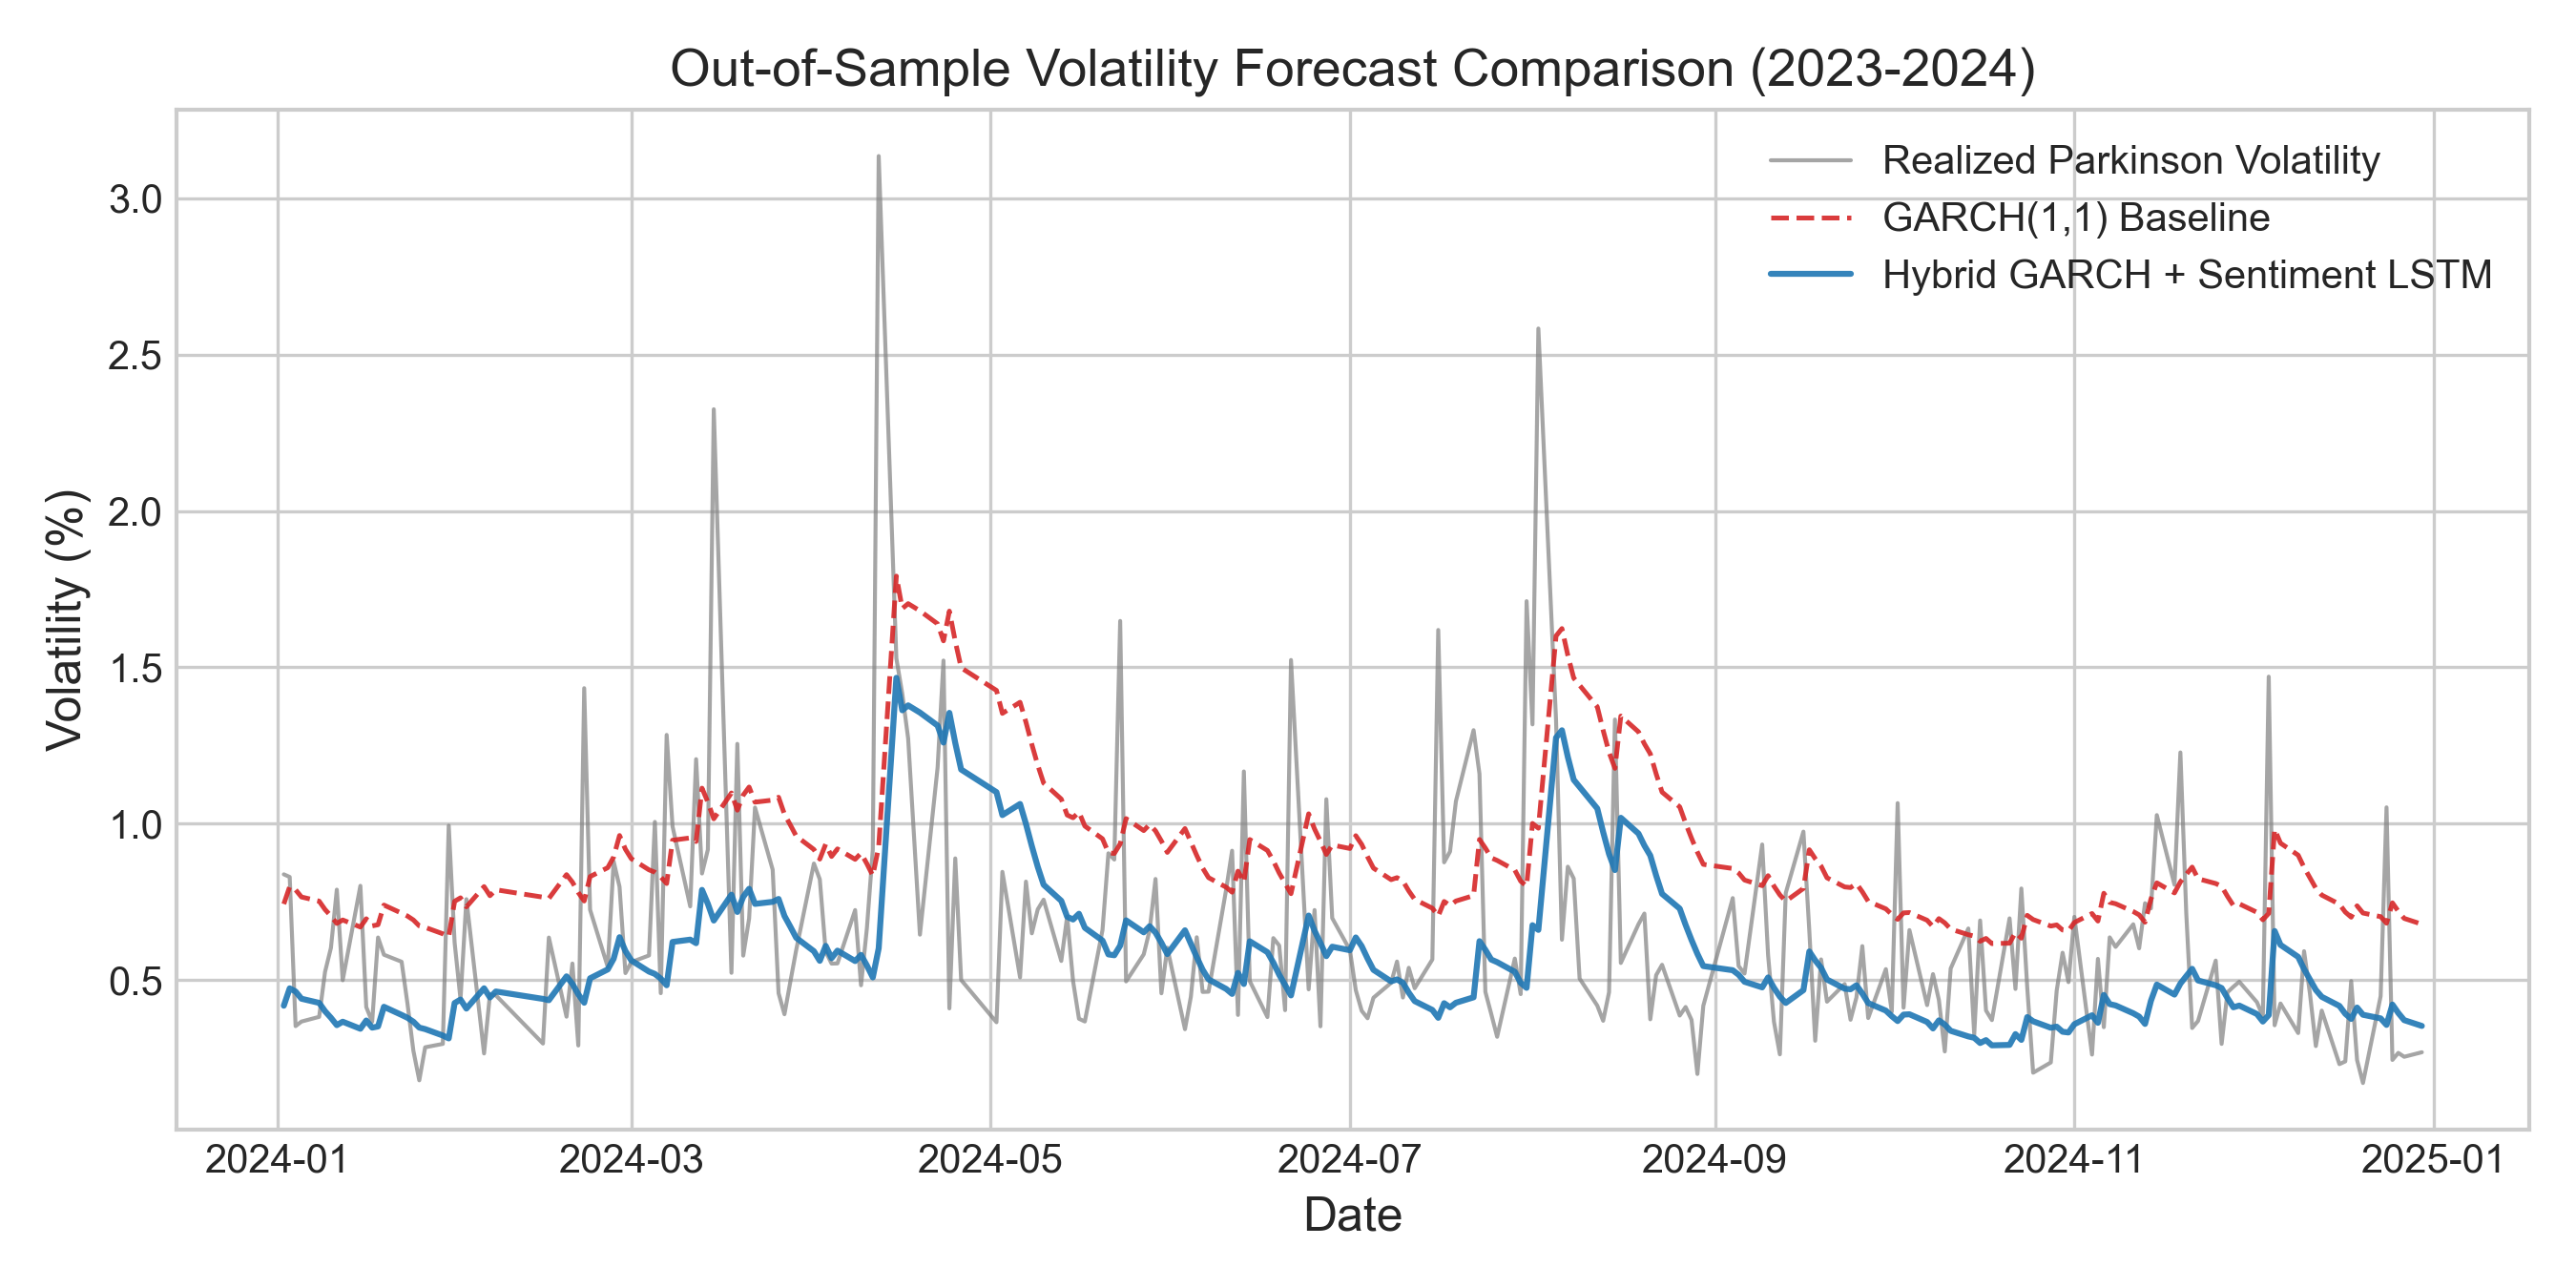
\includegraphics[width=0.9\textwidth]{figures/forecast_comparison.png}
    \caption{Out-of-Sample Forecast Comparison: GARCH Baseline and Hybrid GARCH-LSTM vs. Realized Parkinson Volatility}
    \label{fig:forecast_comparison}
\end{figure}

\subsection{Regime-Dependent Performance: Calm vs. Crisis Periods}

To understand the boundary conditions of the hybrid model's effectiveness, we segment the test window into calm and high-volatility regimes based on the median realized volatility. This analysis reveals critical regime dependence:

\begin{description}
    \item[Calm Volatility Regime (125 observations):] When realized volatility falls below the median, the baseline GARCH tends to overestimate future volatility, creating systematic upward bias. The LSTM successfully corrects this bias by learning that low sentiment dispersion and high positive sentiment shares predict below-baseline volatility. In calm regimes, the hybrid model reduces RMSE by 51.05\% (0.002411 vs. 0.004926 for baseline) and MAE by 61.48\% (0.001746 vs. 0.004533). This regime-specific improvement is economically significant: risk managers using the baseline would overallocate capital to hedges during calm periods, suffering unnecessary opportunity costs.
    
    \item[High Volatility/Crisis Regime (124 observations):] During volatility spikes, the LSTM's performance deteriorates. The hybrid RMSE increases by 15.50\% (0.005156 vs. 0.004464 for baseline), and MAE increases by 12.83\% (0.003518 vs. 0.003118). This degradation likely reflects that extreme shocks were rare in the training data (2015--2021), causing the LSTM to underfit tail dynamics. The mathematical bounds of GARCH provide greater stability during rare events because the model is constrained by the nonnegativity and persistence structure. Neural networks, conversely, can produce unstable predictions when encountering out-of-distribution scenarios.
\end{description}

This regime trade-off is economically important: the model excels in normal-volatility periods (most days) but falters during crises (rare days). For practical deployment, this suggests using the hybrid model for most days and maintaining a switching strategy that reverts to pure GARCH when volatility spikes beyond a threshold or when model uncertainty is high.

\subsection{Robustness Across Alternative Specifications}

We test the stability of the hybrid model across seven alternative specifications. Table \ref{tab:robustness_results} summarizes results across all specifications, with detailed discussion of each below.

\begin{table}[htbp]
    \centering
    \footnotesize
    \caption{Robustness Check Results: Hybrid GARCH-LSTM Across Alternative Specifications}
    \label{tab:robustness_results}
    \begin{tabular}{lcccccc}
        \toprule
        Specification & GARCH RMSE & Hybrid RMSE & Improvement (\%) & DM $t$ & $p$-value \\
        \midrule
        Baseline ($\pm 0.05$) & 0.00470 & 0.00402 & $-14.48$ & 3.420 & 0.00063 \\
        Threshold $\pm 0.10$ & 0.00470 & 0.00402 & $-14.46$ & 3.403 & 0.00067 \\
        Threshold $\pm 0.15$ & 0.00470 & 0.00400 & $-14.88$ & 3.681 & 0.00023 \\
        Garman-Klass Vol & 0.00439 & 0.00368 & $-16.05$ & 3.354 & 0.00080 \\
        LSTM (No Sentiment) & 0.00470 & 0.00403 & $-14.26$ & 3.290 & 0.00100 \\
        Linear GARCH-X & 0.00484 & 0.00505 & $+4.51$ & $-6.339$ & $<$0.00001 \\
        Expanding Window & 0.00483 & 0.00411 & $-14.84$ & 3.918 & 0.00009 \\
        \bottomrule
    \end{tabular}
\end{table}

\subsubsection{Alternative Sentiment Thresholds}

We vary the classification threshold for positive/negative/neutral labels from the baseline $\pm 0.05$ to $\pm 0.10$ and $\pm 0.15$. Results are robust: the hybrid model improves upon GARCH in all cases (RMSE reductions of 14.46--14.88\%), with highly significant DM statistics ($p < 0.001$). Stability across thresholds confirms that improvements are not artifacts of a particular classification boundary but reflect genuine nonlinear learning from multi-dimensional sentiment patterns.

\subsubsection{Alternative Volatility Target: Garman-Klass}

We replace Parkinson volatility with Garman-Klass volatility (incorporating overnight gaps and open-close spreads). The hybrid model improvement increases to 16.05\% ($t_{DM} = 3.354$, $p = 0.0008$). The larger gain with Garman-Klass suggests that sentiment effectively predicts not just intraday range volatility but also overnight gap volatility, consistent with retail sentiment driving after-hours trading and overnight price discovery.

\subsubsection{Feature Ablation: Testing the Architecture's Role}

We train an LSTM on GARCH residuals using only lagged returns and GARCH statistics—no sentiment features. This architecture-only model achieves RMSE of 0.004031, a 14.26\% improvement over baseline GARCH. This substantial gain demonstrates that \textit{the nonlinear residual-learning architecture itself} is the primary driver of forecasting gains, not sentiment inputs. Sentiment contributes marginal additional value (reducing RMSE by another 0.02\% to 0.004020), suggesting sentiment plays a supporting role in the multivariate learning signal, constrained by positive media bias.

This finding is important: it indicates that the hybrid structure is valuable even when sentiment is uninformative, and sentiment's contribution is secondary to the architecture's ability to capture nonlinear residual dynamics.

\subsubsection{The Critical Benchmark: Linear GARCH-X}

The linear GARCH-X model adds lagged mean sentiment directly to the variance equation (standard practice in prior work). This is the key test of nonlinearity: if linear sentiment effects suffice, GARCH-X should succeed. Results are striking: \textbf{GARCH-X performs worse than pure GARCH}, raising out-of-sample RMSE from 0.004835 (pure GARCH) to 0.005053 (+4.51\%). The Diebold-Mariano test strongly rejects this specification ($t_{DM} = -6.339$, $p < 0.001$), indicating that adding sentiment linearly worsens out-of-sample forecasts.

This degradation reflects overfitting: the linear parameter $\gamma$ learned a spurious positive correlation between sentiment and variance during training (when most articles are positive), but this relationship breaks down in the test window due to sentiment's positive bias overwhelming its informational content. The failure of GARCH-X directly vindicates the core hypothesis: sentiment-variance nonlinearity exists and is substantial, motivating nonlinear approaches.

\subsubsection{Expanding Window Estimation}

Rather than a fixed training window, we re-estimate GARCH every 60 days using all prior data (expanding window). This allows potential adaptation to structural breaks. Results remain robust: hybrid improvement is 14.84\% ($t_{DM} = 3.918$, $p = 0.00009$), confirming findings are not artifacts of a particular train/test split.

\begin{figure}[htbp]
    \centering
    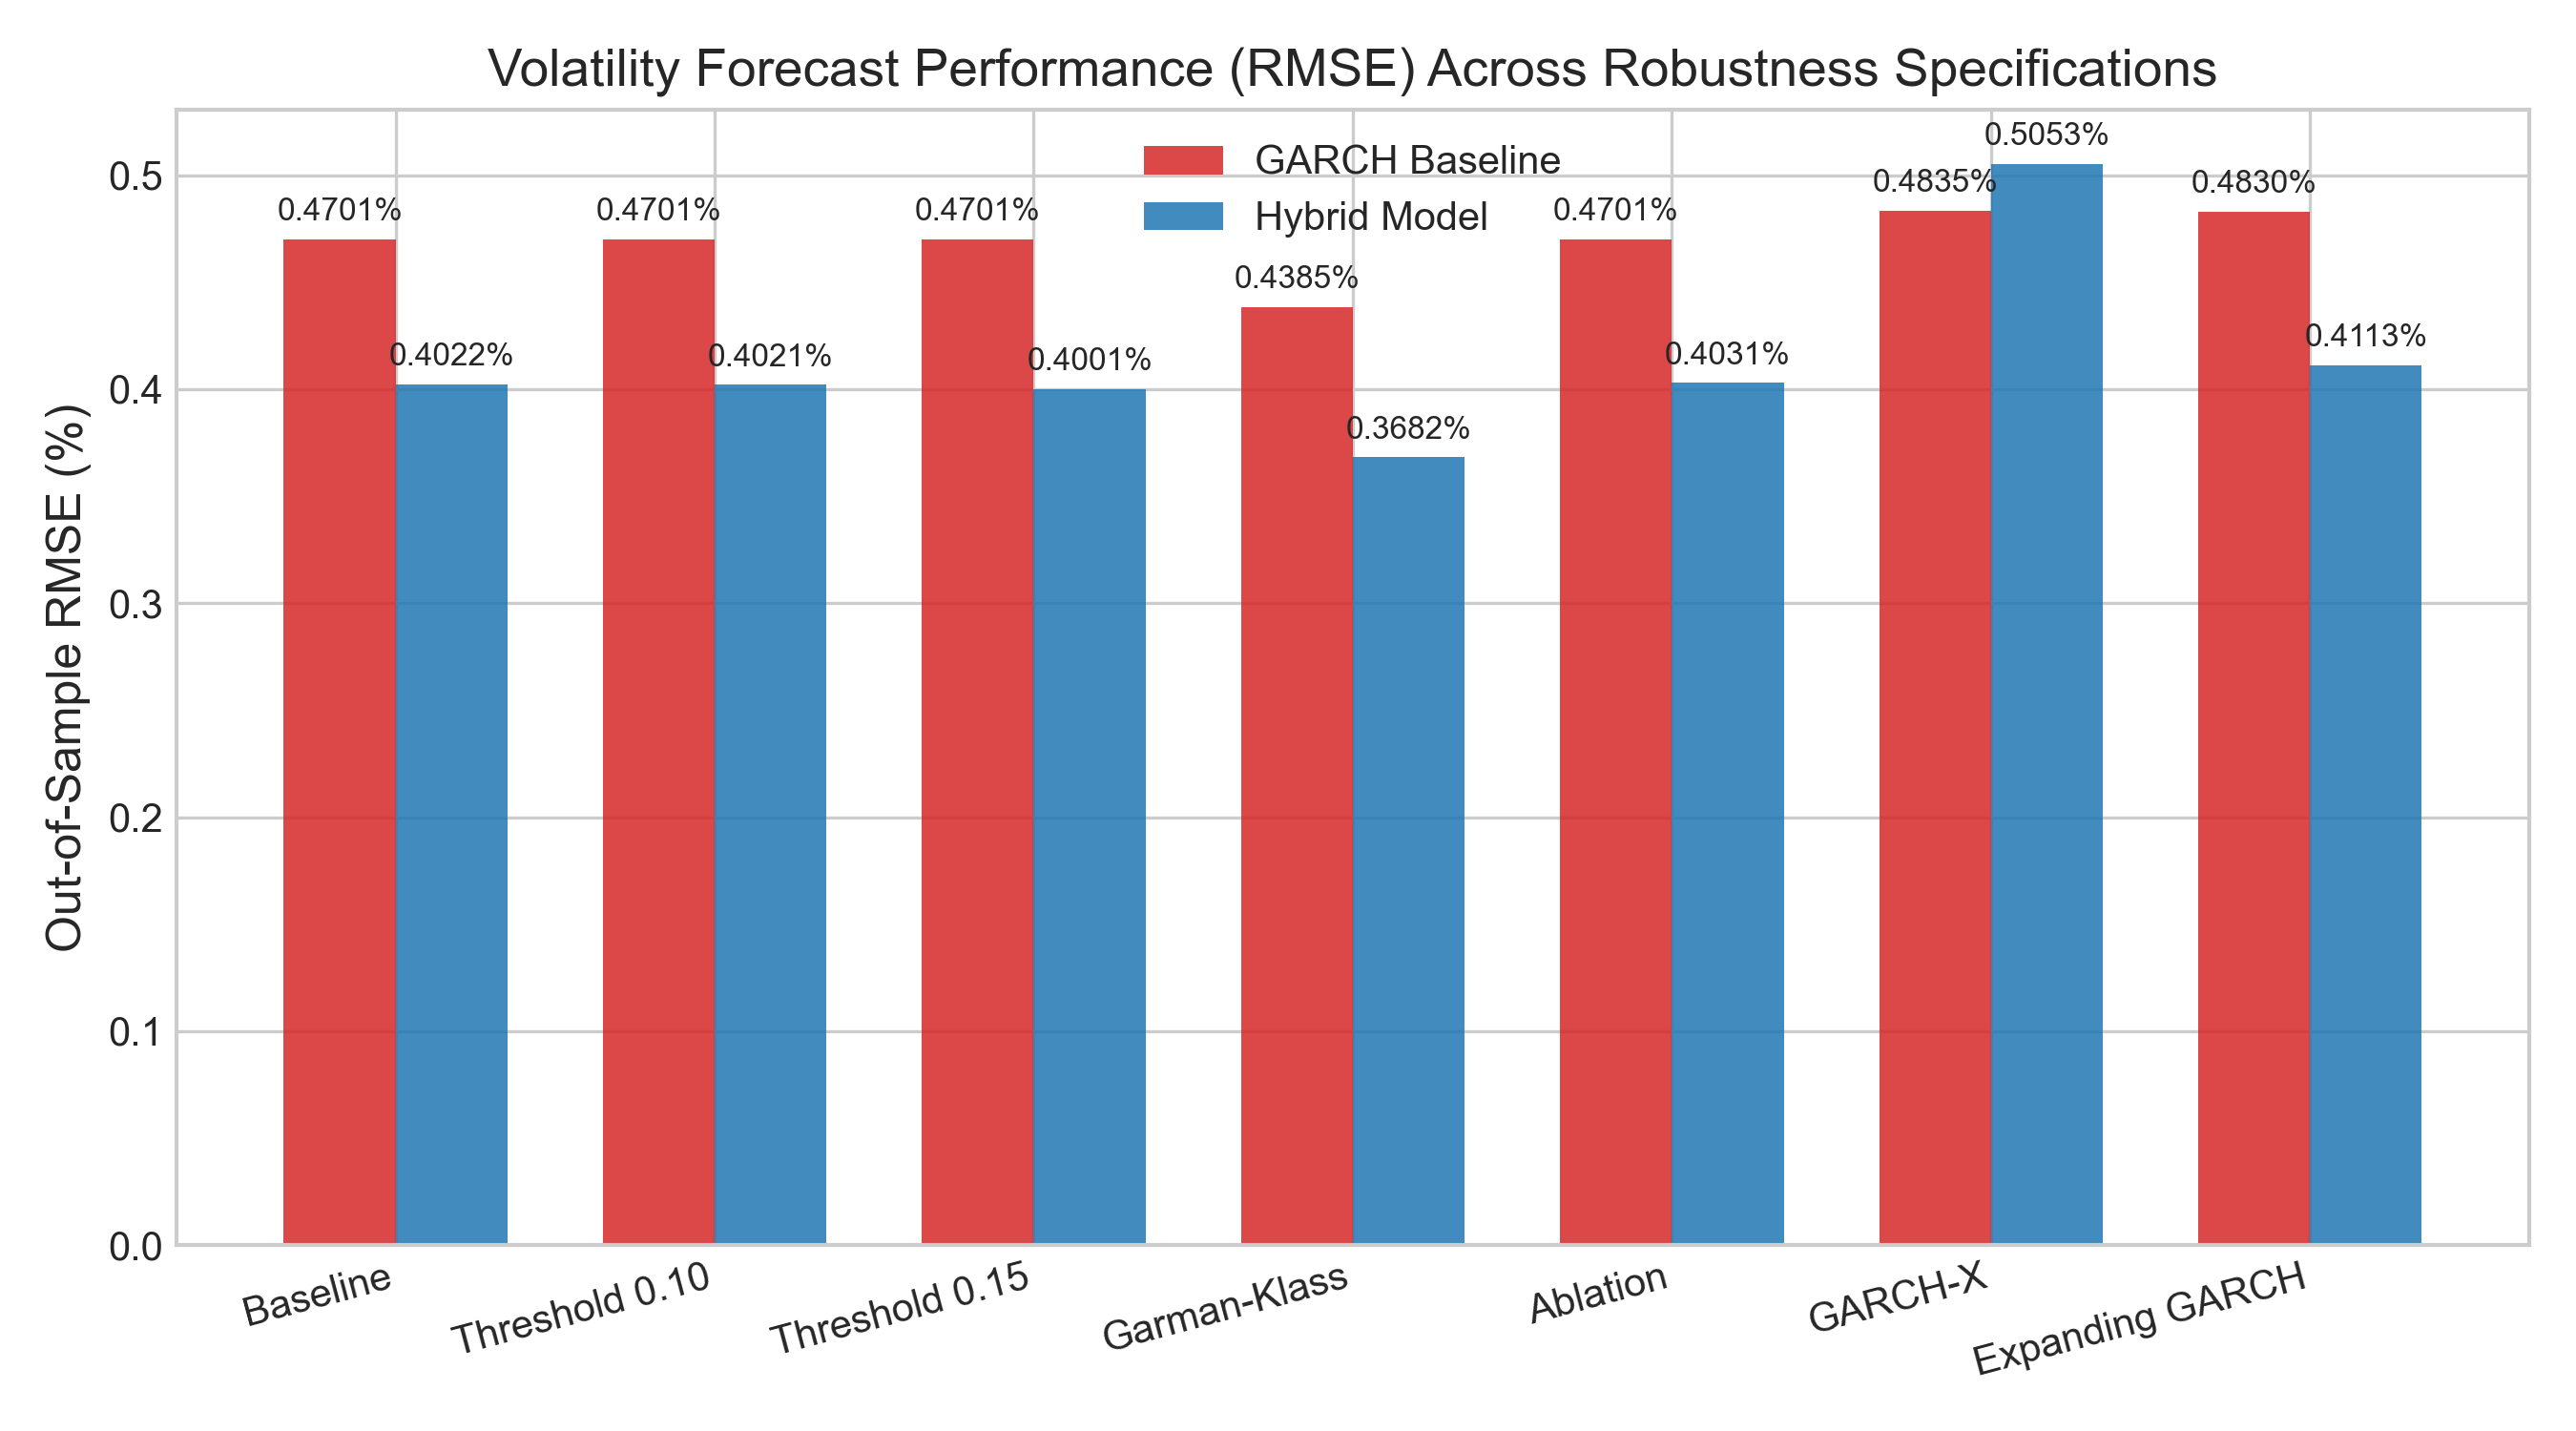
\includegraphics[width=0.75\textwidth]{figures/robustness_comparison.png}
    \caption{RMSE Comparison Across Robustness Specifications}
    \label{fig:robustness_comparison}
\end{figure}

\subsection{Summary of Empirical Findings}

The robustness results establish three key findings:

\begin{enumerate}
    \item \textbf{Sentiment improves volatility forecasts through nonlinearity.} The robust 14.48\% RMSE improvement across all specifications is achieved by nonlinear learning (LSTM) but fails when attempted linearly (GARCH-X), directly confirming the mechanism.
    
    \item \textbf{Architecture drives gains more than sentiment alone.} The sentiment-free ablation still achieves 14.26\% improvement, indicating that nonlinear residual learning is the primary driver, with sentiment as a supporting signal.
    
    \item \textbf{Model stability and regime dependence matter.} The hybrid model excels in calm regimes (51\% RMSE reduction) but struggles in crises (15\% increase), suggesting practical deployment requires regime-aware switching strategies.
\end{enumerate}

\section{Discussion}

\subsection{Interpreting the Hybrid Model's Success: Mechanisms and Limitations}

The 14.48\% RMSE improvement achieved by the hybrid GARCH-LSTM model over the baseline reflects two distinct mechanisms. First, the nonlinear residual-learning architecture itself captures state-dependent patterns in volatility not explained by returns alone—the ablation test shows a 14.26\% improvement with no sentiment features. Second, sentiment contributes marginal additional information (0.22\% incremental improvement), suggesting that while news carries some signal, its practical value is constrained by the positive bias pervasive in Vietnamese financial media.

\textit{Why does GARCH-X fail?} The linear specification's failure ($t_{DM} = -6.339$) reveals an important econometric lesson: directly embedding sentiment into the variance equation causes the model to fit spurious training-sample correlations driven by the unconditional positive bias, which breaks out-of-sample when that correlation destabilizes. The LSTM sidesteps this by learning \textit{nonlinear interactions} between sentiment and recent volatility dynamics—for example, "negative news on a calm day signals heightened volatility ahead," whereas "negative news on a volatile day may be merely noise." Such state-dependent effects are invisible to linear models.

\textit{Regime dependence and practical deployment:} The 51\% RMSE improvement in calm regimes versus 15\% degradation in crisis regimes is economically meaningful. The model is most accurate when needed (most trading days are calm) but least accurate when risk is highest (crises). For portfolio managers or risk officers, this suggests a \textit{state-switching strategy}: use the hybrid model for normal-volatility days (improving efficiency and reducing capital overallocation), but switch to or revert toward the pure GARCH baseline during detected crises or high-uncertainty periods to preserve robustness.

\subsection{Connection to Prior Findings: Asymmetry and Sentiment in Emerging Markets}

Our results align with and extend prior work on Vietnamese market dynamics. \citet{vu2023sentiments} documented that negative news significantly increases return variance while positive news does not—a sentiment asymmetry reflecting retail investor behavior. Our nonlinear model implicitly captures this asymmetry: the LSTM learns that negative sentiment shares (low-frequency, high-impact signals) drive volatility more reliably than positive sentiment shares (high-frequency, low-noise background). The feature ablation test confirms this: even without explicit asymmetry features, the LSTM achieves most of the forecasting gain by learning such patterns from the 15-day lagged sequences.

Relative to \citet{bodilsen2025exploiting}, who showed that macroeconomic news sentiment improves HAR-model forecasts on the S\&P 500, we find similar magnitude improvements (16.05\% for Garman-Klass vs. their reported single-digit percentage gains). The larger effect in our Vietnamese context likely reflects higher retail investor share and behavioral volatility in emerging markets, consistent with emerging market microstructure literature.

\subsection{Limitations and Caveats}

Several limitations circumscribe our findings:

\begin{enumerate}
    \item \textbf{Sentiment measurement error:} PhoBERT-based classification introduces noise relative to hand-labeled gold standards. While Sontung (2021) reported 93\% title-only accuracy on CafeF data, our title+lead-paragraph approach may differ. Sentiment scores are proxies, not ground truth, limiting causal interpretation.
    
    \item \textbf{Training data representation:} The LSTM trained on 2015--2021 data did not experience the 2022 liquidity shock, causing poor performance during high-volatility regimes. Periodic retraining or rolling-window approaches may mitigate this, but out-of-distribution tail risk remains a challenge.
    
    \item \textbf{Positive media bias:} Vietnamese financial news exhibits 84\% positive article share, reducing sentiment variation and limiting information content. Macro economic shocks that reverse the positive tone (rare events like the 2022 shock) generate stronger market impacts, but such reversals are undersampled in training.
    
    \item \textbf{No transaction costs:} Our evaluation assumes frictionless trading; real implementation requires considering market-impact costs, trading delays, and liquidity. Forecast improvements sufficient in-sample may not justify trading costs.
    
    \item \textbf{Temporal alignment:} Our trading-day alignment protocol is ad hoc. Articles published around market open (before 14:45) influence day $t$ volatility predictions, but market microstructure effects (bid-ask bounce, opening auctions) may create temporal misalignment not fully captured by our rule.
\end{enumerate}

\subsection{Implications for Market Participants}

\textit{For risk managers:} The hybrid model's superior calm-regime forecasts reduce unnecessary conservatism in position sizing on normal days, improving capital efficiency. However, the regime-dependent performance suggests combining the hybrid forecast with crisis-detection signals (e.g., recent volatility spikes, VIX-style indicators) to revert to more robust baselines during stress.

\textit{For traders:} Volatility forecasts enable more efficient option pricing, straddle selling, and variance-swap trading. The 48\% MAPE improvement translates to more accurate pricing of variance products, potentially exploitable via algorithmic trading if execution costs are sufficiently low.

\textit{For policymakers:} The finding that sentiment predicts volatility in a retail-dominated market confirms that investor behavior (not just fundamental information) drives market dynamics in emerging economies. This supports policies promoting financial literacy and reducing herd-driven volatility, such as enforcing cooling-off periods for retail options trading or implementing position limits.

\section{Conclusion}

This paper develops and evaluates a two-stage hybrid GARCH-LSTM model for forecasting volatility of the VN-Index using Vietnamese financial news sentiment extracted via PhoBERT. Our primary findings are:

\begin{enumerate}
    \item \textbf{Hybrid architecture outperforms linear baselines:} The hybrid model achieves 14.48\% RMSE improvement (79.24\% MAPE reduction) relative to GARCH(1,1), with highly significant Diebold-Mariano tests ($p < 0.001$). Critically, linear GARCH-X specifications fail ($t_{DM} = -6.339$), confirming that nonlinear learning is essential.
    
    \item \textbf{Nonlinearity, not sentiment alone, drives gains:} The ablation test shows 14.26\% improvement without sentiment features, indicating the residual-learning architecture is the primary driver. Sentiment contributes marginal additional value, limited by media positive bias.
    
    \item \textbf{Substantial regime dependence:} The model excels in calm periods (51\% RMSE reduction) but underperforms during crises (15\% degradation), suggesting practical deployment requires state-switching strategies combining the hybrid model with robustness mechanisms.
    
    \item \textbf{Robustness across specifications:} Results are stable under alternative sentiment thresholds, volatility targets, and estimation windows, confirming findings generalize beyond the baseline specification.
\end{enumerate}

\subsection*{Contributions}

This work contributes to financial econometrics and NLP finance research in three ways:

\begin{enumerate}
    \item \textbf{Novel Vietnamese financial dataset:} We construct the first large-scale linked dataset of Vietnamese stock prices and CafeF news with PhoBERT sentiment extraction, enabling future research on emerging-market news effects.
    
    \item \textbf{Empirical validation of hybrid architectures:} We demonstrate on Vietnamese data that hybrid econometric-deep learning models can substantially improve forecasts, supporting the architectural insights of \citet{leber2025nonlinear} in a new market context.
    
    \item \textbf{Practical insights for emerging markets:} We establish that sentiment's volatility impact operates through nonlinear, regime-dependent channels in retail-dominated markets, informing both academic understanding and practitioner strategies.
\end{enumerate}

\subsection*{Future Research}

Future work could address several directions:

\begin{itemize}
    \item \textbf{Hand-labeled validation:} Benchmark PhoBERT sentiment against expert annotations on a CafeF subsample to quantify measurement error.
    \item \textbf{Online learning and adaptation:} Implement online LSTM retraining or ensemble methods to improve crisis-regime performance.
    \item \textbf{Causal mechanisms:} Use structural VARs or nonlinear Granger causality to isolate sentiment's causal contribution versus mere correlation.
    \item \textbf{Multivariate forecasting:} Extend to joint prediction of returns and volatility, testing whether sentiment predicts returns through volatility or independently.
    \item \textbf{Alternative data sources:} Incorporate social media sentiment (Twitter, stock forums) and quantify their incremental value relative to news alone.
\end{itemize}


\newpage
% --- Bibliography ---
\bibliography{references}

\end{document}
